\subsection{概要}
検証器の実装にあたっては,\ref{compcert}節で説明したCompCertを拡張する
形で実装した.本研究では,下図のConstraint Generator, Constraint
Reducer, Type-error Slicer を実装した.

\begin{figure}[H]
  \centering
  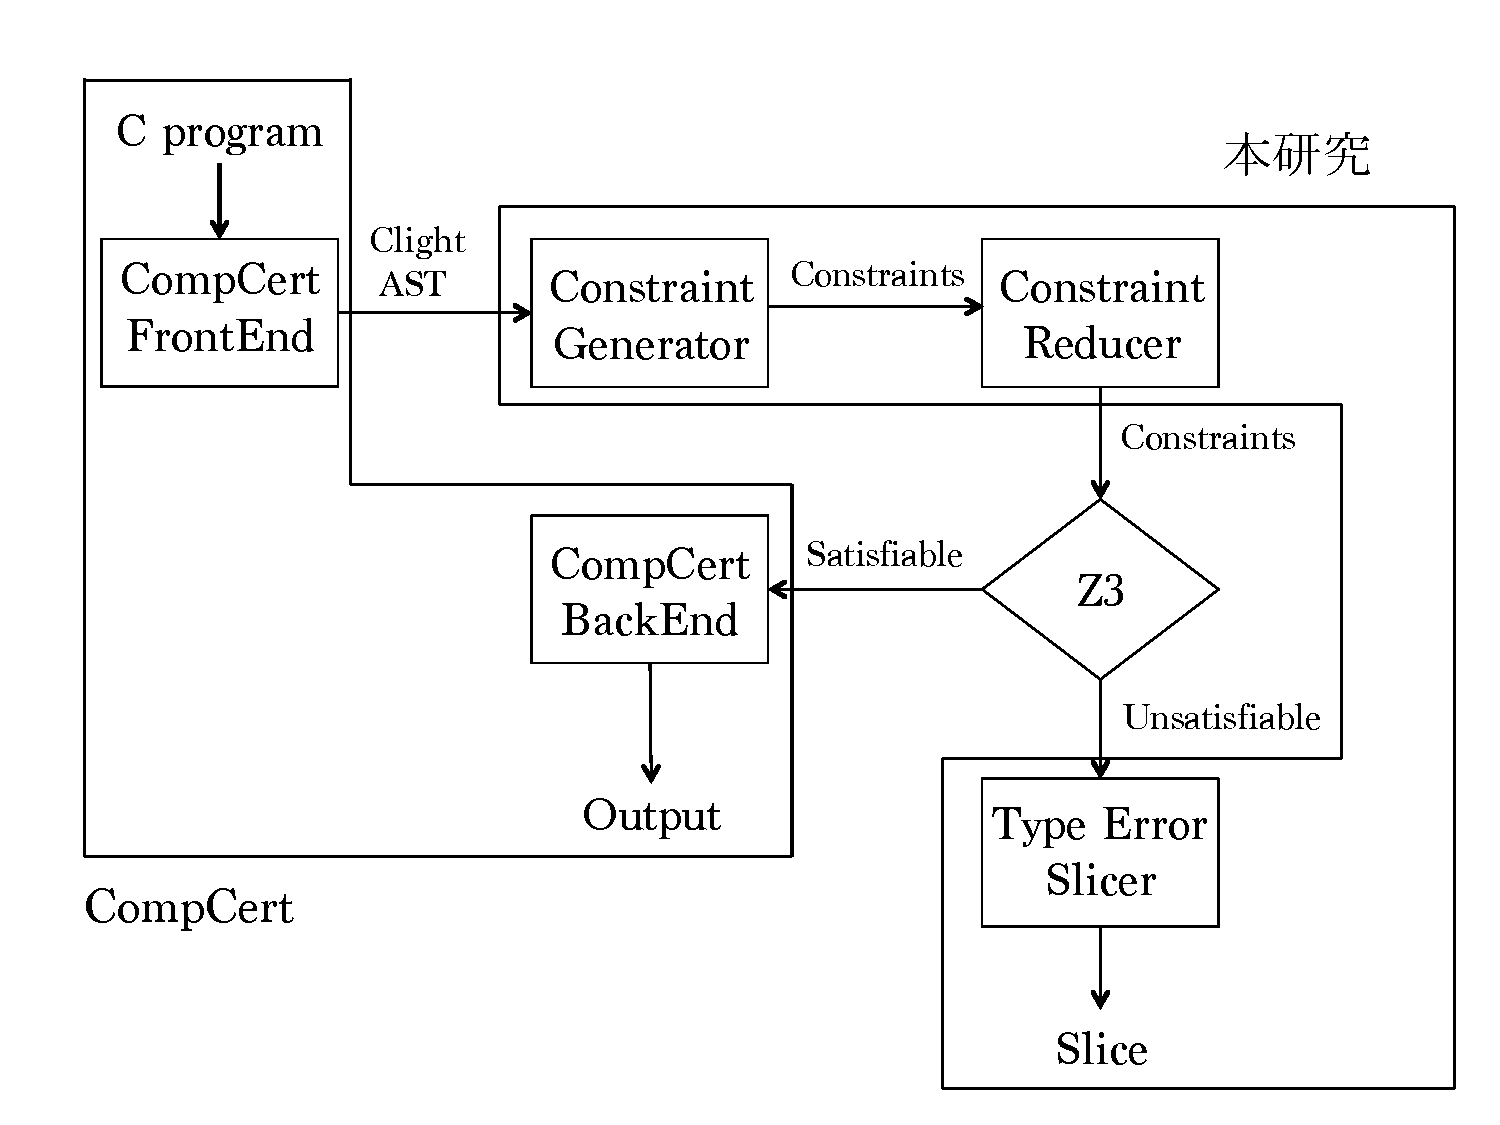
\includegraphics[width=0.9\textwidth]{verifier.pdf}
  \label{impl}
  \caption{実装の全体図}
\end{figure}

CompCertは,C言語のプログラムを受け取るとまず中間言語であるClightに変換す
る.検証器はそのClightの抽象構文木を入力として,型付け規則(図
\ref{typing_stmt})に従い制約式を生成する.そしてその制約式をSMTソルバが解
くことのできる形に変換した後,SMTソルバに渡す.制約式が充足可能であればプ
ログラムに型がつき,メモリ操作に関する誤りが無いことがわかるため,Clihgt
ASTをそのままCompCertに返す.充足不能の場合,SMTソルバはunsat coreを返す.
unsat coreとは,充足不能の原因となっている制約式の部分集合である.型エラー
スライサーは,unsat coreを受け取り,unsat coreに含まれている制約式を生成
した命令の行番号を,スライスとして出力する.


\subsection{制約生成}
この節では,制約生成(Generate)について説明する.まず,扱う制約式につい
て定義する.

\begin{definition}[制約式]
  制約式を図\ref{constr}のように定義する.
\end{definition}
\begin{figure}[htbp]
  \centering
  $
  \begin{aligned}
    c\ (constraints)\ ::=
    \ & \mathtt{Le} (o_{1},\,o_{2},\,loc)\ \\
    |\ &\mathtt{Lt}(o_{1},\,o_{2},\,loc)\ \\
    |\ &\mathtt{Eq}(o_{1},\,o_{2},\,loc)\ \\
    |\ &\mathtt{Empty}(id,\,n,\,loc)\ \\
    |\ &\mathtt{Teq}((id,\,n)\ list,\ (id,\,n)\ list,\ loc)
  \end{aligned}
  $
  \caption{制約式}
  \label{constr}
\end{figure}

各制約式の$loc$は,どの命令から生成された制約式なのかを記録しておくための
情報である.制約式が充足不能となった場合,unsat coreに含まれている制約式
がどの命令から生成されたものなのかを調べ,その命令の行番号を抽出するため
に使用する.

\texttt{Le}は$o_{1} \le o_{2}$,\texttt{Lt}は$o_{1} < o_{2}$,
\texttt{Eq}は$o_{1} = o_{2}$にそれぞれ対応している.\texttt{Empty}は,構
造体の名前を表す$\mathit{id}$,同じ名前でも違う所有権をもつ構造体を区別す
る識別子$n$を受け取る.構造体中の所有権が全て0であるという制約式を表して
いる.\texttt{Teq}は,構造体同士の所有権が等しいという制約式を表している.
各引数がリストになっているのは,型の定義で新しく追加した\texttt{Tplus}を
引数として取れるようにするためである.これにより,構造体を足し算したもの
同士が等しいという制約式も表すことができる.

制約生成の流れは,以下の通りである.入力としてClightプログラムの抽象構文
木を受け取る.図\ref{clight_program}で定義したように,プログラムは関数定
義のリストになっている

\begin{enumerate}
  \item 関数定義から関数環境を生成する
  \item 1の操作を各関数定義に適用する
  \item 引数,局所変数を型環境に追加する
  \item 関数本体に対して所有権に関する制約式を生成する
  \item 3, 4を各関数定義に適用する
\end{enumerate}

まず,関数定義から関数環境を生成する.関数環境は,関数名から関数の型への
写像で定義されている.関数の型\texttt{function}は,引数の型$t_{1}\
\mathit{list}$と,関数実行後の引数の型$t_{2}\ \mathit{list}$,返り値の型
$t$の組で定義されている.返り値の型$t$と引数の型の$t_{1}\ \mathit{list}$
は,関数定義に使われている返り値の型$t$と引数のリスト$\mathit{dcl}_1$をそ
のまま使えば良い.この際,引数の型にポインタ型が含まれている場合,フレッ
シュな所有権変数を割り当てる.また,構造体が含まれている場合も,フレッシュ
な識別子を割り当てる.そして,実行前の引数の型にフレッシュな所有権変数と
構造体にフレッシュな識別子を割り当てたものを関数実行後の引数の型とする.
この操作を各関数定義に対して行う.

\begin{example}[関数環境の生成]
例えば,
\begin{verbatim}
  struct list {
      struct list *next;
      int n
  };

  void free_list(struct list *l)
\end{verbatim}
のように,構造体と関数が定義されている場合,\texttt{free\_list}には,
\begin{verbatim}
function(
  struct(list,
         [(list, comp_ptr(list, 0, Ovar(0)));
          (list, int)]),
  struct(list,
         [(list, comp_ptr(list, 1, Ovar(1)));
         (list, int)]),
  void)
\end{verbatim}
のような型がつく.1引数目の\texttt{Tstruct}が\texttt{free\_list}の引数の
型,2引数目の\texttt{Tstruct}が\texttt{free\_list}を実行した後の引数の型,
3引数目の\texttt{void}が\texttt{free\_list}の返り値の型になっている.この
ように,関数実行後の引数の型は,実行前の引数の型内に含まれる識別子にフレッ
シュなものを割り当てた型にする.そして,(\texttt{free\_list},
\ \texttt{function(...)})を関数環境に追加する.\label{example1}
\end{example}

関数環境の生成後,関数本体について制約式を生成する.まず,関数定義の引数
$\mathit{dcl}_{1}$,局所変数$\mathit{dcl}_{2}$から型環境を生成する.型環
境は,変数名から変数の型への写像で定義されているので,
$\mathit{dcl}_{1},\,\mathit{dcl}_2$をそのまま使えば良い.この際,関数環境
の時と同様に,型内に所有権や構造体の識別子が含まれている場合は,他と被ら
ないように新しい識別子を割り当てる.また,関数本体実行前の局所変数の所有
権は全て0でないといけないという制約式をこの段階で生成する.

この型環境を最初の型環境として,関数本体$s$に対して,図\ref{typing_stmt}
に従い所有権に関する制約式を生成する.基本的には,型付け規則の前提部分を
制約式にしていく.例えば,前提部分の$o = 0$などは,そのまま$\texttt{Eq}(o,\
\texttt{OConst}(0))$とすればよい.

$\texttt{empty}(t)$は,型$t$内の所有権が全て$0$であるということを表してい
る.そこで,型$t$内の所有権が全て$0$であるという制約式を生成する関数
\texttt{empty\_type}を定義する.\texttt{int}や\texttt{float}など,所有権
が割り当てられていない型は,全ての所有権が$0$になっているとみなして良い.
$\texttt{pointer}(t,\ o)$は,$\texttt{Eq}(o,\ \texttt{Oconst}(0))$という
制約式を生成した後,$t$に対して再帰的に\texttt{empty\_type}を適用していく.
$\texttt{struct}(\mathit{id},\ \mathit{fl})$は,$\mathit{fl}$の各要素に対
して\texttt{empty\_type}を適用する.$\texttt{comp\_ptr}(\mathit{id}, n,
o)$は,\texttt{pointer}と同様に$\texttt{Eq}(o,\ \texttt{Oconst}(0))$とい
う制約式を生成した後,参照先に対して所有権が$0$であるという制約式を生成す
る.しかし,\texttt{comp\_ptr}は,再帰を含む構造体内での自己参照をしてい
るポインタのため,\texttt{empty\_type}をそのまま適用していくと,無限ルー
プに陥ってしまう.そこで,図\ref{constr}で定義した$\texttt{Empty}(id, n,
loc)$で,$\texttt{comp\_ptr}$の参照先の所有権が全て$0$である,ということ
を表す.

$t_{1} + t_{2}$は,型$t_1$と型$t_2$を足した型を表している.型同士の足し算
は,所有権同士の足し算として定義されている.そこで,型$t_1$内の所有権と型
$t_2$内の所有権を足す関数\texttt{add\_type}を定義する.基本的には,同じ型
同士しか足し算は行うことができない.所有権が割り当てられていない
\texttt{int}などに関しては,\texttt{empty\_type}と同様に何もせず,そのま
ま$t_{1}$を返す.$\texttt{pointer}(t_{1}',\ o_{1})$と
$\texttt{pointer}(t_{2}',\ o_{2})$に関しては,$t_{1}'$と$t_{2}'$に対して
再帰的に\texttt{add\_type}を適用し,その返り値を$t'$とすると,
$\texttt{pointer}(t',\ \texttt{Oplus}(o_{1},\ o_{2}))$を返す.
\texttt{struct}同士の足し算に関しては,まず構造体の名前が一緒かどうかを確
認する.同じ場合は,フィールドリストの各要素に対して\texttt{add\_type}を
適用する.名前が違う場合は,足し算を行うことはできないので,エラーを返す.
\texttt{comp\_ptr}同士の足し算に関しても,まず同じ構造体内のポインタであ
るかどうかを確認する.また,\texttt{empty\_type}と同様に
\texttt{comp\_ptr}の参照先に関して再帰的に\texttt{add\_type}を実行すると,
無限ループに陥ってしまうため,$\texttt{Tplus}$を使い,\texttt{comp\_ptr}
同士の足し算を表す.

更に,\texttt{comp\_ptr}はポインタ型のため,
$\texttt{comp\_ptr}(\mathit{id},\ n,\ o_{1})$と$\texttt{pointer}(t,\
o_{2})$の足し算を定義することができる.この場合は,\texttt{comp\_ptr}を構
造体を参照しているポインタと読み替える.まず,
$\texttt{comp\_ptr}(\mathit{id},\ n,\ o_{1})$を一回展開する.展開するには,
構造体の名前$\mathit{id}$と構造体内の所有権を区別する識別子$n$を使う.ま
ず$\mathit{id}$と$n$の組で,今までに展開されているかどうかを調べる.展開
されている場合は,以前展開された構造体をそのまま使う.展開されていない場
合,構造体内の\texttt{pointer}と\texttt{comp\_ptr}の所有権と識別子をフレッ
シュなものに書き換えた新たな構造体をつくり,その構造体を参照先にする.こ
の時,$\mathit{id}$と$n$の組が新しく作った構造体を参照しているという情報
を記録しておく.これにより,$\mathit{id}$と$n$の組は常に同じ構造体に展開
されることになる.

$t_{1} = t_{2}$は,型$t_{1}$と型$t_{2}$が等しいという条件を表している.型
同士の等しさは,所有権同士の等しさで定義されている.そこで,型$t_{1}$内の
所有権と型$t_{2}$内の所有権が等しいという制約式を生成する関数
\texttt{eq\_type}を定義する.定義は,\texttt{empty\_type}や
\texttt{add\_type}と同様にすればよい.所有権が割り当てられていない型に関
しては,何もしない.\texttt{pointer}同士に関しては,再帰的に
\texttt{eq\_type}を適用する.\texttt{comp\_ptr}同士に関しては,再帰的に適
用すると無限ループに陥るため,\texttt{Teq}を使い,等しさを表す.
\texttt{comp\_ptr}と\texttt{pointer}に関しては,\texttt{comp\_ptr}を構造
体を参照しているポインタとみなす.\texttt{comp\_ptr}を展開する際の処理も
同様である.

\begin{example}[制約生成]
構造体の定義は例\ref{example1}と同じとする.\\
型環境が
\begin{verbatim}
  l: pointer(struct(list,
                    [(list, comp_ptr(list, 0, Ovar(0)));
                     (list, int)]),
                    Ovar(1))
\end{verbatim}
のもとで,
\begin{verbatim}
  free(l)
\end{verbatim}
を実行すると,実行後の型環境が
\begin{verbatim}
  l: pointer(struct(list,
                    [(list, comp_ptr(list, 0, Ovar(0)));
                     (list, int)])struct(list,
                    [(list, comp_ptr(list, 0, Ovar(0)));
                     (list, int)]),
                    Ovar(2))
\end{verbatim}
になり,制約式として
\begin{verbatim}
  Eq(Ovar(1), Oconst(1), loc);
  empty_type(struct(list,
                    [(list, comp_ptr(list, 0, Ovar(0)));
                     (list, int)]));
  Eq(Ovar(2), Oconst(0), loc);
\end{verbatim}
が生成される.更に\texttt{empty\_type}からは,
\begin{verbatim}
  Eq(Ovar(0), Oconst(0), loc);
  Empty(list, 0, loc);
\end{verbatim}
が生成される.
\texttt{loc}には,\texttt{free(l)}のプログラム中での行番号が入る.
\end{example}

関数本体に対して制約式の生成が終わると,関数本体実行後の型環境が得られる.
この型環境内に含まれる引数の型は,関数環境内に追加されている関数実行後の
引数の型と一致しなければならない.また,関数本体実行後には関数の局所変数
の所有権は全て0になっていなければならない.この2つの条件に関しても制約式
を生成する.この操作を各関数定義に対して適用する.

以上の操作によって得られた制約式を集めたものが制約式の集合となる.この制
約式の集合をSMTソルバで解く.\texttt{Le},\texttt{Lt},\texttt{Eq}は不等
式の形をしているため,そのままSMTソルバで解くことができるが,
\texttt{Empty},\texttt{Teq}はこのままではSMTソルバは解くことができない.
そのため,SMTソルバに解ける形に変換する必要がある.
